\chapter{Avaliação} \label{ch:evaluation}

Este Capítulo apresenta resultados comparativos da solução desenvolvida com a 
aplicação original. A Seção \ref{sect:methodology} apresenta detalhes da 
metodologia de avaliação e a Seção \ref{sect:results} disserta sobre os 
resultados.


\section{Metodologia de Avaliação} \label{sect:methodology}

Os experimentos foram realizados no Parque Computacional de Alto Desempenho 
(PCAD) da UFRGS. Eles ocorreram nos nós de computação draco, sua 
configuração é mostrada na Tabela \ref{tab:draco_config}.


\begin{table}[H]
%\small
\centering
\begin{tabular}{l l} \toprule
\textbf{Parâmetro}  &  \textbf{Configuração} \\ 
\midrule
Processador     & 2 x Intel Xeon E5-2630 (Q1'12) Sandy Bridge, 2,5 GHz  
\\
Número de Núcleos    & 16 núcleos (8 por CPU)  \\
Memória       & 64 GB DDR3 RAM   \\
\end{tabular}
\caption{Configurações dos nós draco.}
\label{tab:draco_config}
\end{table}


A Figura \ref{fig:experiment_arch} exibe a arquitetura que foi seguida durante 
os experimentos. Como os experimentos com o Spark acessam dados direto do HDFS, 
primeiramente executamos o Hadoop. Um dos nós era responsável por executar o 
\emph{namenode} e também executava uma instância de \emph{datanode}. Os demais 
executavam apenas instâncias de \emph{datanodes}.


\begin{figure}[ht]
\centerline{
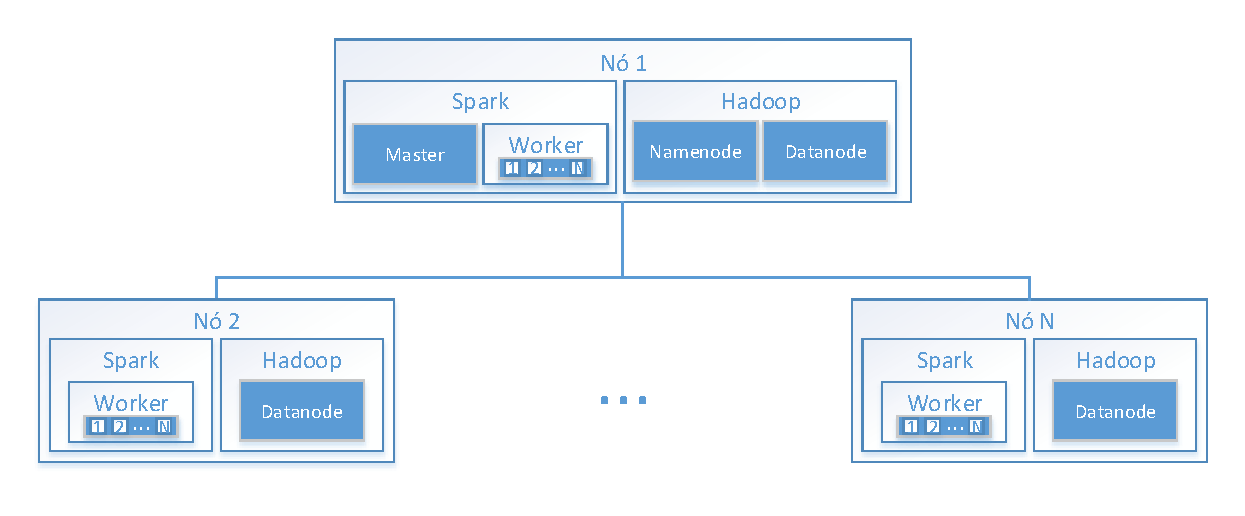
\includegraphics[width=0.9\textwidth]{./img/experiments_arch.pdf}}
 \caption{Arquitetura de aplicações durante os experimentos.}
 \label{fig:experiment_arch}
\end{figure}


O gerenciador de cluster utilizado foi o do próprio Spark ao invés do YARN. 
Essa decisão foi tomada durante os testes pois seus logs mostraram 
informações mais claras sobre o que estava ocorrendo. A instânciação dele foi 
similar àquela utilizada no Hadoop, um nó executou como \emph{mestre} e 
\emph{trabalhador} enquanto os demais executaram apenas como 
\emph{trabalhadores}. 

Cada \emph{trabalhador} do Spark instancia N \emph{executores}, responsáveis 
por processar tarefas. Cada um destes possui uma quantidade de cores e uma 
quantidade de memória dedicada. Durante os experimentos, parametrizamos a 
\emph{Engine} para que cada \emph{trabalhador} instanciasse 15 
\emph{executores}, cada um com 2 cores e 4 GB de memória para processamento de 
tarefas.

Realizamos testes com um nó, utilizando a aplicação original, um, dois e três 
nós, utilizando a aplicação modificada. Cada teste foi executado 
aproximadamente 30 vezes (a salvo algum problema de execução em alguma 
repetição) para garantir a confiabilidade de seus resultados. 


\section{Experimentos e Resultados} \label{sect:results}

A carga de trabalho dos experimentos já no formato CSV (entrada para a fase de 
pré-processamento no StarVZ), tinha um somatório de 12 GB. Ela consiste em 
rastros de execução de uma aplicação cholesky e foi escolhida pois era a maior
entrada que tínhamos no momento. O tamanho de cada um dos arquivos pode ser 
visualizado na Tabela \ref{tab:input_sz}.

\begin{table}[H]
\centering
\begin{tabular}{l c} \toprule
\textbf{Arquivo}  &  \textbf{Tamanho} \\ 
\midrule
state.csv	& 6.8 GB \\
variables.csv  	& 2.5 GB \\
link.csv       	& 304 MB \\
dag.csv        	& 270 MB \\
entities.csv	& 73 KB \\
events.csv	& 1.8 GB \\
\textbf{Total}  & 12 GB  \\
\end{tabular}
\caption{Detalhamento da carga de trabalho.}
\label{tab:input_sz}
\end{table}

Durante a implementação, optou-se por manter o processamento de Entities
no formato sequencial pois esse arquivo armazena apenas informações de 
plataforma e por isso, costuma não passar da ordem de tamanho de KB. Podemos 
observar que isso se confirma nesta carga de trabalho.


Foram executadas 30 repetições em cada teste, todavia, os experimentos com o 
Spark apresentaram problemas em algumas execuções. Com um nó, 3 execuções foram 
interrompidas e com dois e três nós, uma. Nesses casos, consideramos apenas 
aquelas que processaram com sucesso (27, 29 e 29 repetições, respectivamente). 

A Figura \ref{fig:total_full} mostra a média do tempo total de execução dos 
experimentos e o desvio padrão no topo da barra, em função do nível de 
paralelismo (quantidade de \emph{Executores}) em cada nó. A execução 
original, de forma sequencial, levou em média, 1489,02 segundos para completar 
o processamento. Já as execuções com a aplicação adaptada para utilizar o 
Spark, com apenas um nó levou em média 708,17 segundos, com dois, 460,81 
segundos e com três, 385,44 segundos. Isso consiste em um \emph{speedup} de 
respectivamente 2,10x, 3,23x e 3,86x em relação ao original.

\begin{figure}[ht]
\centerline{
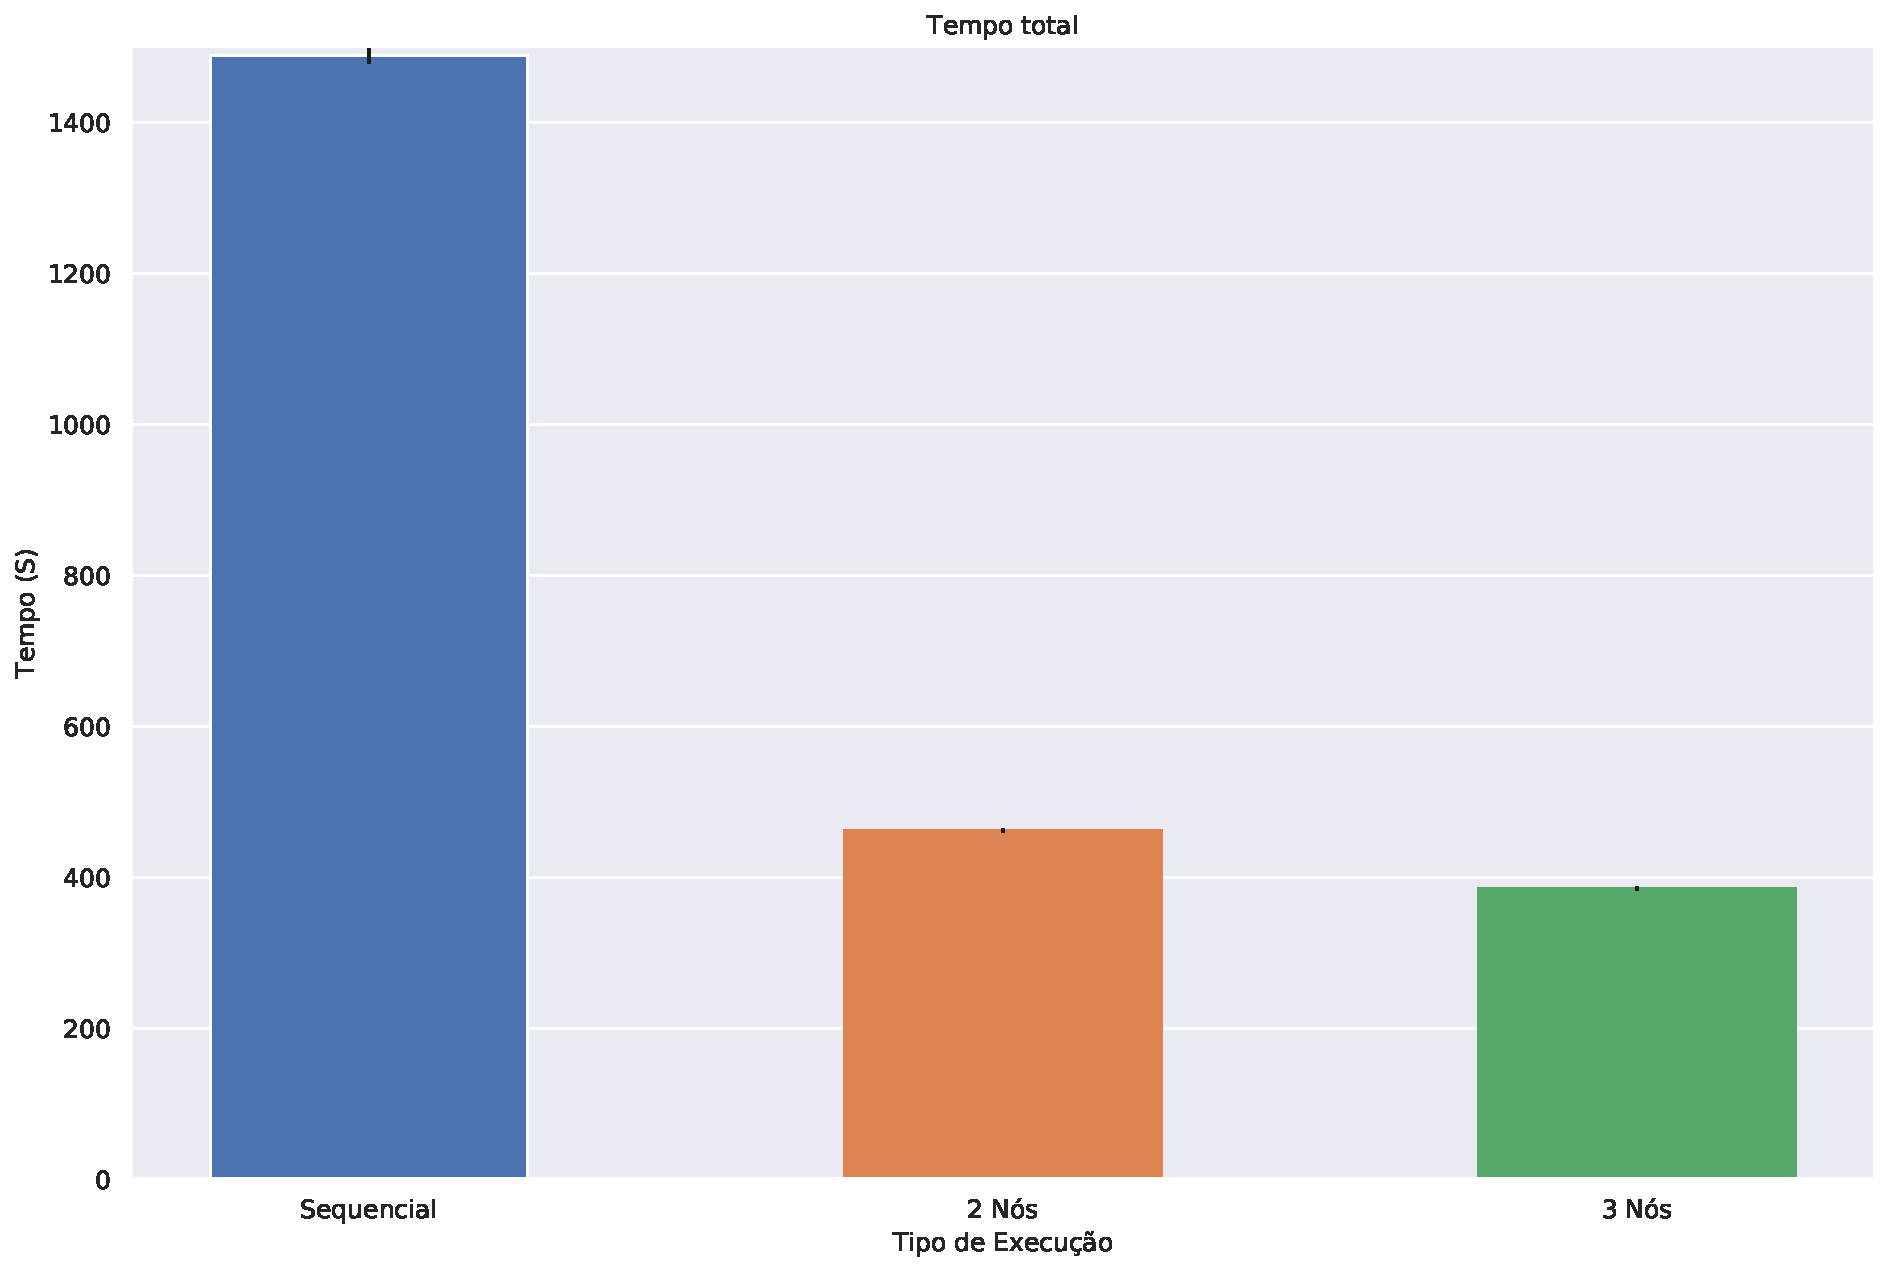
\includegraphics[width=0.8\textwidth]{./img/total.pdf}}
 \caption{Tempo total de execução da aplicação.}
 \label{fig:total_full}
\end{figure}


Segmentamos a análise pelas etapas exibidas na Figura 
\ref{fig:spark-starvz-flow}, seus tempos de execução podem ser visualizados na 
Figura \ref{fig:total_step} e consultados com mais detalhes na Tabela 
\ref{tab:total_step}. Analisando os resultados e o código, conseguimos 
separar as etapas em quatro grupos.

O primeiro e mais trivial deles, é o grupo em que não houve praticamente 
nenhuma alteração de código e tempo de execução. É o caso do tratamento de 
Entities, que foi apenas convertido para uma tabela Spark para posterior 
gravação no HDFS.

\begin{figure}[H]
\centerline{
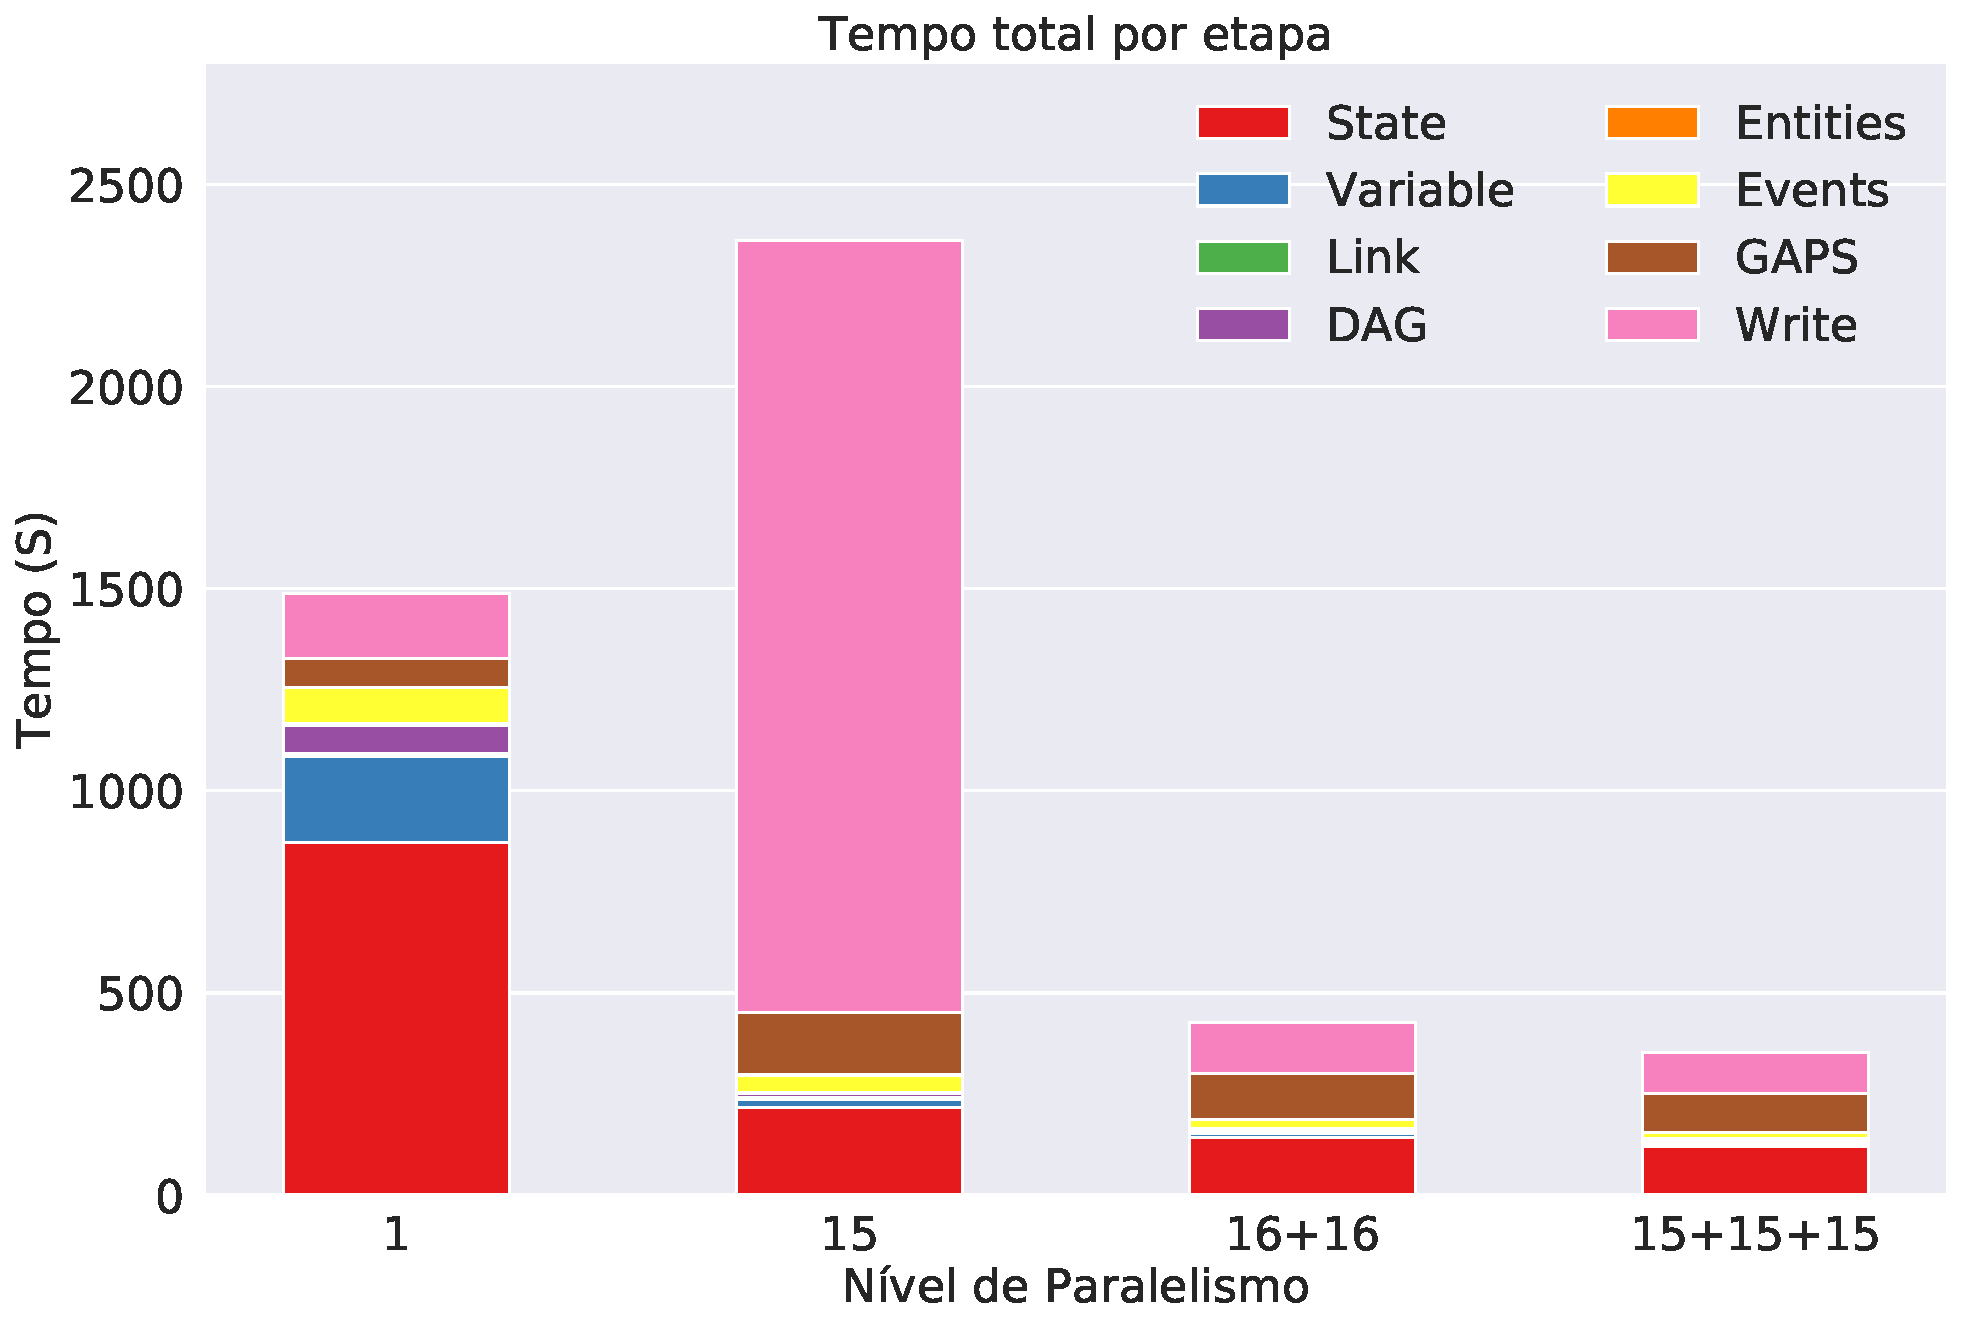
\includegraphics[width=0.8\textwidth]{./img/total_step.pdf}}
 \caption{Tempos de execução segmentados por etapas.}
 \label{fig:total_step}
\end{figure}


\begin{table}[ht]
\centering
\begin{tabular}{l c c c c} \toprule
\textbf{Etapa}  & \textbf{1} & \textbf{15} & \textbf{15+15} & 
\textbf{15+15+15}\\ 
\midrule
State		& 873.31 & 215.93 & 142.15 & 119.20\\
Variable  	& 210.77 & 21.17  & 10.44  & 7.50 \\
Link      	& 8.93   & 4.59   & 3.84   & 3.53 \\
DAG        	& 69.14  & 10.10  & 7.58   & 6.76 \\
Entities	& 3.07   & 2.42   & 2.31   & 2.30 \\
Events		& 89.87  & 42.68  & 22.65  & 15.91\\
GAPS		& 71.51  & 110.83 & 110.83 & 95.22\\
Write		& 162.19 & 211.06 & 125.40 & 102.87\\
\end{tabular}
\caption{Tempos médios de execução, em segundos.}
\label{tab:total_step}
\end{table}

O segundo grupo identificado, foram manipulações que executaram apenas 
Transformações no Spark \cite{ref:sparkbook}. Estas constroem um plano de 
operações a serem aplicadas nos dados, todavia, a \emph{Engine} só irá 
executá-lo quando estritamente necessário (quando uma Ação for realizada). 
Neste grupo enquadram-se as tabelas que observou-se um \emph{speedup} muito 
grande, como é o caso de Variable que apresentou 9,95x, 20,18x, 28,10x 
comparando-se as execuções com Spark com a execução Sequencial. DAG também teve 
ganhos consideráveis, apresentendo \emph{speedups} de 6,84x, 9,12x e 10,22x. Os 
ganhos de Link foram menos significativos, pois seu tempo original já é pequeno, 
concluímos que ele pertence a este grupo pela análise do código de seu 
tratamento.

O terceiro grupo identificado foram transformações que de alguma forma ativaram 
uma Ação no Spark. Tais operações fazem com que a \emph{Engine} efetivamente 
manipule os dados \cite{ref:sparkbook} não sendo do tipo \emph{Lazy} como as 
Transformações. Esse grupo consiste nos tratamentos de State e Events, nos 
quais tivemos um ganho inferior ao segundo grupo. Os ganhos observados para 
Events foram de 2,10x, 3,96x e 5,64x, enquanto que para State tivemos 4,04x, 
6,14x e 7,32x.

O último grupo, corresponde apenas ao Cálculo de GAPS. Essa operação foi 
levantada durante a implementação como um ponto de atenção, devido ao seu tempo 
ter aumentado de forma considerável em experimentos locais. Olhando para os 
tempos de execução temos, em segundos, 71,51 na execução sequencial, 154,03 na 
execução com 1 nó utilizando Spark, 110,83 na execução com 2 nós e 95,22 
utilizando 3 nós. Acreditamos que isso seja decorrente de Ações Spark 
realizadas em tabelas geradas por junções de forma recursiva, que é o que esta 
etapa faz. Para identificar o ponto exato que causa essa perda de desempenho, 
são necessários mais testes.

Por fim, temos a escrita dos dados no sistema de arquivos distribuído. Nessa 
etapa pode-se observar que o ganho não é tão grande pois é nela que todos os 
planos de transformações montados nas etapas anteriores serão efetivamente 
executados sobre os dados. Pode-se observar, tanto na Tabela 
\ref{tab:total_step} quanto na Figura \ref{fig:total_step} que o tempo de 
execução com o Spark apenas em um nó (15 executores) é pior do que a execução 
sequencial. Depois dela, temos \emph{speedups} singelos de 1,29x e 1,57x.

Portanto, podemos concluir que a portagem do arcabouço StarVZ para executar 
sobre o Spark gerou ganhos consideráveis. Há outras diversas avaliações para 
serem realizadas, algumas serão enumeradas no próximo Capítulo.



